\section{The Second Variation}

\subsection{Definition and Conditions on Local/Global Minimum}

For a \emph{function}, we have
\[
    f\pqty{\vb{x} + \epsilon \vb*{\xi}} - f\pqty{\vb{x}} = \epsilon \vb*{\xi} \vdot \grad f + \frac{\epsilon^2}{2} \xi_i \xi_j H_{ij} \pqty{\vb{x}} + \bigO \pqty{\epsilon^3}.
\]

So a stationary point \(\vb{x} = \vb{a}\) is a local minimum, if \(H_{ij} \pqty{\vb{x}}\) is positive-definite, or equivalently, all eigenvalues of \(H_{ij}\) are positive.

In this section, we aim to generalise this idea to a functional.

For a functional
\[
    F \bqty{y} = \int_{\alpha}^{\beta} f\pqty{y, y', x} \dd{x}
\]
where
\begin{equation}
    \label{eq:boundary-eqn}%
    y \in \contClassSymb = \set{y \in \contClass{2} \pqty{\ccintv{\alpha}{\beta}}}{y\pqty{\alpha} = a, y\pqty{\beta} = b}.
\end{equation}

Consider \(y + \epsilon \xi\) where \(\xi\) is now our variation, with \(y + \epsilon \xi \in \contClassSymb\). In particular, \(\xi\pqty{\alpha} = \xi\pqty{\beta} = 0\). (We called \(\epsilon \xi = \var{y}\) before.) Taylor expanding, we get
\begin{align*}
    f\pqty{y + \epsilon \xi, y' + \epsilon \xi', x} &= f\pqty{y, y', x} + \epsilon \xi \bqty{\pdv{f}{y} - \dv{x} \pdv{f}{y'}} + \epsilon \dv{x} \pqty{\xi \pdv{f}{y'}} \\
    &\phantom{=} + \frac{1}{2} \epsilon^2 \bqty{\xi^2 \pdv[2]{f}{y} + 2 \xi \xi' \pdv{f}{y}{y'} + \xi'^2 \pdv[2]{f}{{y'}}} + \bigO\pqty{\epsilon^3}.
\end{align*}

This gives
\[
    F\bqty{y + \epsilon \xi} - F\bqty{y} = \epsilon \int_{\alpha}^{\beta} \xi \fdv{F}{t} \dd{x} + \epsilon^2 \var[2]{F\bqty{y, \xi}} + \bigO\pqty{\epsilon^3}
\]
where the boundary term vanishes due to our initial conditions in \autoref{eq:boundary-eqn}, and where we denote
\[
    \var[2]{F\bqty{y, \xi}} = \frac{1}{2} \int_{\alpha}^{\beta} \pqty{\xi^2 \pdv[2]{f}{y} + 2 \xi \xi' \pdv{f}{y}{y'} + \xi'^2 \pdv[2]{f}{{y'}}} \dd{x}.
\]

Writing \(2 \xi \xi' = \pqty{\xi^2}'\), using integration by parts (and that the boundary terms vanishes by \autoref{eq:boundary-eqn}), we have
\begin{equation}
    \label{eq:second-variation}%
    \begin{aligned}
        \var[2]{F\bqty{y, \xi}} &= \frac{1}{2} \int_{\alpha}^{\beta} \pqty{\xi^2 \pdv[2]{f}{y} + 2 \xi \xi' \pdv{f}{y}{y'} + \xi'^2 \pdv[2]{f}{{y'}}} \dd{x} \\
        &= \frac{1}{2} \int_{\alpha}^{\beta} \bqty{\xi^2 \pqty{\pdv[2]{f}{y} - \dv{x} \pdv{f}{y}{y'}} + \pqty{\xi'}^2 \pdv[2]{f}{{y'}}} \dd{x}.
    \end{aligned}
\end{equation}

\begin{definition}[Second Variation]
    We define the \emph{second variation} by \autoref{eq:second-variation}, as
    \[
        \var[2]{F\bqty{y, \xi}} = \frac{1}{2} \int_{\alpha}^{\beta} \bqty{\xi^2 \pqty{\pdv[2]{f}{y} - \dv{x} \pdv{f}{y}{y'}} + \pqty{\xi'}^2 \pdv[2]{f}{{y'}}} \dd{x}
    \]
\end{definition}

Recall that if \(\vb{H} \pqty{\vb{x}}\) is positive-definite for \emph{all} \(\vb{x}\), then \(f\pqty{\vb{x}}\) is \emph{convex}, and any stationary point is guaranteed to be a \emph{global minimum}. We have a similar analogue for functional derivatives.

\begin{theorem}[``Convexity'' Condition and Stationary Points for Functionals]
    If
    \[
        \var[2]{f\bqty{y, \xi}} \geq 0
    \]
    for \emph{all} \(y \in \contClassSymb\) and all ``allowed'' \(\xi\pqty{x}\) (i.e. \(y + \xi \in \contClassSymb\), in other words, \(\xi\) is \(\contClass{2}\) and \(\xi\pqty{\alpha} = \xi\pqty{\beta} = 0\)), then \(y = y_0\) is a global minimum of \(F\) in \(\contClassSymb\), if \(y_0 \in \contClassSymb\) satisfies the Euler--Lagrange equation.
\end{theorem}

Notice that the class of functions \(\contClassSymb\), as defined in \autoref{eq:boundary-eqn}, is indeed convex by the definition of a convex set.

\begin{example}[Geodesics in the Euclidean Plane]
    Recall we have the length functional
    \[
        F\bqty{y} = \int_{\alpha}^{\beta} \sqrt{1 + \pqty{y'}^2} \dd{x}.
    \]

    Using \autoref{eq:second-variation}, since we have
    \[
        \pdv[2]{f}{y} = \pdv{f}{y}{y'} = 0,
    \]
    and that
    \[
        \pdv[2]{f}{{y'}} = \pqty{1 + \pqty{y'}^2}^{- \flatfrac{3}{2}},
    \]
    we get
    \[
        \var[2]{F\bqty{y, \xi}} = \frac{1}{2} \int_{\alpha}^{\beta} \pqty{\xi'}^2 \pqty{1 + \pqty{y'}^2}^{- \flatfrac{3}{2}} \dd{x} \geq 0.
    \]

    So the solution to the Euler--Lagrange equation, which is a straight line, is indeed a global minimum of the distance between two points.
\end{example}

But usually our functionals does not have this \emph{global} condition. Now, suppose \(y_0 \in \mathcal{C}\) satisfies Euler--Lagrange equations, then similar to the question we asked on the Hessian before, we may use the \emph{local} behaviour of the second variation to determine its property.

\begin{theorem}[Second Variation and Stationary Points for Functionals]
    If \(y_0 \in \contClassSymb\) satisfies the Euler--Lagrange equation, then \(y_0\) is a:
    \begin{itemize}
        \item \emph{local minimum} of \(F\), if \(\var[2]{F\bqty{y_0, \xi}} > 0\), for all non-trivial allowed \(\xi\);
        \item \emph{not a local minimum} of \(F\), if \(\var[2]{F\bqty{y_0, \xi}} < 0\), for some allowed \(\xi\).
    \end{itemize}
\end{theorem}

\begin{figure}[ht!]
    \centering
    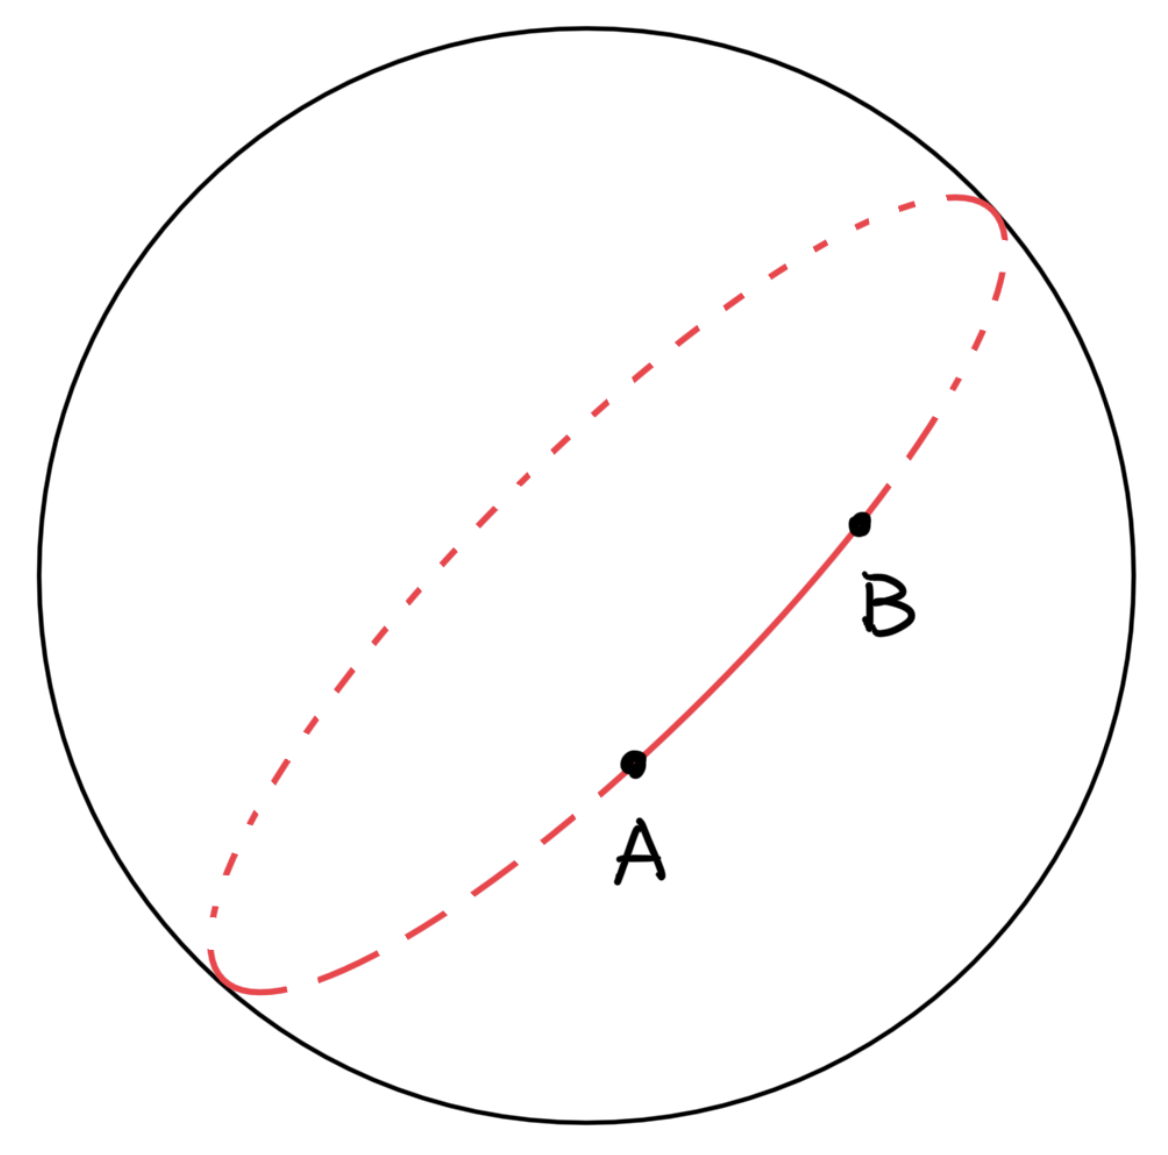
\includegraphics[width=0.5\linewidth]{fig/geodesics-sphere.png}
    \caption{Geodesics on the Sphere}
    \label{fig:geodesics-on-the-sphere}%
\end{figure}

\begin{example}[Geodesics on the Sphere]
    The geodesics between points \(A\) and \(B\) on the sphere is a segment of a great circle (i.e. diameter) through the points \(A\) and \(B\).

    Note there are in fact two segments, as shown in \autoref{fig:geodesics-on-the-sphere}, and the shorter path has \(\var[2]{F} > 0\) for all non-trivial \(\xi\), giving a local minimum. In fact, this is a global minimum, but from this criteria alone we cannot conclude that.

    The longer path has \(\var[2]{F} < 0\) for some \(\xi\), so it cannot be a local minimum.

    (Note that if \(A, B\) are antipodal (i.e. lie directly opposite each other), then we in fact have \(\var[2]{F} \geq 0\) for all \(\xi\), allowing us to use the condition analogue to the convexity condition.)
\end{example}

\begin{theorem}[Legendre Condition]
    \label{thm:legendre-condition}%
    If \(y_0 \in \contClassSymb\) satisfies the Euler--Lagrange equation, then a \emph{necessary} condition for a local minimum is
    \begin{equation}
        \label{eq:legendre-condition}%
        \pqty{\pdv[2]{f}{{y'}}}_{y = y_0} \geq 0
    \end{equation}
    for all \(x \in \ccintv{\alpha}{\beta}\).
\end{theorem}

\begin{proof}[(Outline)]
    If this quantity were negative at some point \(x = x_0 \in \ccintv{\alpha}{\beta}\), then this allows us to choose some allowed \(\xi\), such that \(\xi\) is only non-zero near \(x_0\) and \(\xi'\) is large while \(\xi\) is small, and this will make \autoref{eq:second-variation} negative, hence not a local minimum.
\end{proof}

\begin{example}[Application of Legendre Condition]
    Consider the functional
    \[
        F\bqty{y} = \int_{-1}^{1} x \sqrt{1 + \pqty{y'}^2} \dd{x}.
    \]

    Then
    \[
        \pdv[2]{f}{{y'}} = x \pqty{1 + \pqty{y'}^2}^{-\flatfrac{3}{2}}
    \]
    and hence this violates \autoref{eq:legendre-condition} for \(x < 0\). Therefore, any solution to the Euler--Lagrange equation cannot be a local minimum.
\end{example}

\begin{definition}[Simplification of Second Variation Notation]
    Let \(y_0 \in \contClassSymb\) be a solution to the Euler--Lagrange equation. We denote
    \[
        \var[2]{F\bqty{y_0, \xi}} = \frac{1}{2} \int_{\alpha}^{\beta} \bqty{\rho \xi'^2 + \sigma \xi^2} \dd{x}
    \]
    where
    \begin{equation}
        \label{eq:second-variation-parameter}%
        \rho = \rightbar{\pdv[2]{f}{{y'}}}_{y = y_0} \qand \sigma = \pqty{\pdv[2]{f}{y} - \dv{x} \pdv{f}{y}{y'}}_{y = y_0}.
    \end{equation}
\end{definition}

Then Legendre Condition stated that \(\rho \geq 0\) is necessary for \(y_0\) to be a local minimum.

\begin{proposition}[Sufficient Condition for Local Minimum]
    If \(\rho > 0\), and \(\sigma \geq 0\) on \(\oointv{\alpha}{\beta}\), then any solution to the Euler--Lagrange equation is guaranteed to be a local minimum.
\end{proposition}

\begin{proof}
    Clearly, \(\var[2]{F} \geq 0\) for all \(\xi\).
    
    If \(\var[2]{F} = 0\) for some \(\xi\), then \(\xi'\) has to vanish on the interval \(\oointv{\alpha}{\beta}\). This means \(\xi\) is a constant. With the boundary conditions in \autoref{eq:boundary-eqn}, \(\xi\) must be identically zero.

    So if \(\xi\) is non-trivial, then \(\var[2]{F} > 0\) strictly.
\end{proof}

\begin{example}[Brachistochrone]
    Recall in \autoref{ex:brachistochrone-curve} that we discussed the minimisation of the time functional
    \[
        T = \int_{0}^{x_B} f \dd{x}
    \]
    where
    \[
        f = \sqrt{\frac{1 + \pqty{y'}^2}{-y}}.
    \]

    Suppose that \(y\) satisfies the Euler--Lagrange equation, i.e. \(y\) is a cycloid. Then
    \[
        \pdv{f}{y'} = \frac{y'}{\sqrt{-y \pqty{1 + \pqty{y'}^2}}}
    \]
    and
    \[
        \pdv{f}{y} = \frac{f}{-2y}.
    \]

    Hence,
    \[
        \rho = \pdv[2]{f}{{y'}} = \frac{1}{\sqrt{\pqty{-y} \pqty{1 + \pqty{y'}^2}^3}} > 0.
    \]

    For \(\sigma\), we have
    \[
        \pdv{f}{y}{y'} = -\frac{1}{2y} \pdv{f}{y'}
    \]
    and
    \[
        \pdv[2]{f}{y} = \frac{3f}{4y^2}.
    \]

    So we have (using that \(y\) is a solution to the Euler--Lagrange equation)
    \begin{align*}
        \sigma &= \pdv[2]{f}{y} - \dv{x} \pdv{f}{y}{y'} \\
        &= \pdv[2]{f}{y} - \frac{y'}{2 y^2} \pdv{f}{y'} + \frac{1}{2y} \pdv{f}{y} \\
        &= \frac{3f}{4 y^2} - \frac{{y'}^2}{2 y^2 \sqrt{\pqty{-y} \pqty{1 + \pqty{y'}^2}}} - \frac{f}{4y^2}\\
        &= \frac{1}{2 \sqrt{\pqty{-y} \pqty{1 + \pqty{y'}^2}}} \\
        &> 0
    \end{align*}
    as well.

    Therefore, we have shown that the cycloid is indeed a local minimum of \(T\).
\end{example}

\subsection{Eigenvalue Problem of Second Variation}

In general, we integrate by parts using \autoref{eq:second-variation-parameter} (c.f. \autoref{eq:sturm-liouville}) to get
\begin{equation}
    \label{eq:second-variation-sturm}%
    \var[2]{F\bqty{y_0, \xi}} = \frac{1}{2} \int_{\alpha}^{\beta} \xi \mathcal{L} \xi \dd{x} + \frac{1}{2} \bqty{\rho \xi \xi'}_{\alpha}^{\beta} = \frac{1}{2} \int_{\alpha}^{\beta} \xi \mathcal{L} \xi \dd{x},
\end{equation}
where we define
\[
    \mathcal{L} = - \dv{x}\pqty{\rho \dv{x}} + \sigma.
\]

Consider the Sturm--Liouville problem, i.e. the eigenvalue problem (c.f. \autoref{eq:eigenvalue-problem})
\begin{equation}
    \label{eq:eigenvalue-problem-variation}%
    \mathcal{L} \eta = \lambda w \eta
\end{equation}
with \(\eta\pqty{\alpha} = \eta\pqty{\beta} = 0\), where \(w > 0\) on \(\oointv{\alpha}{\beta}\).

\begin{proposition}[Existence of Negative Eigenvalue implies Not Local Minimum]
    If \autoref{eq:eigenvalue-problem-variation} admits a negative eigenvalue \(\lambda\), then \(y_0\) is not a local minimum.
\end{proposition}

\begin{proof}
    Let \(\eta\) be an eigenfunction, and set \(\xi = \eta\) in \autoref{eq:second-variation-sturm}, we have
    \[
        \var[2]{F\bqty{y_0, \eta}} = \frac{1}{2} \int_{\alpha}^{\beta} \eta \mathcal{L} \eta \dd{x} = \frac{\lambda}{2} \int_{\alpha}^{\beta} w \eta^2 \dd{x} < 0
    \]
    so this cannot be a local minimum.
\end{proof}

The converse is true as well.

\begin{proposition}[All Eigenvalues Positive implies Not Local Minimum]
    If \autoref{eq:eigenvalue-problem-variation} are all positive, then \(y_0\) is a local minimum.
\end{proposition}

\begin{proof}
    Let \(\lambda_i\) be the \(n\)th eigenvalue, and \(y_n\pqty{x}\) is the \(n\)th eigenfunction to the problem \autoref{eq:eigenvalue-problem-variation}. From \textit{Methods}, we know that the set of functions \(\Bqty{y_n}\) form a complete set for the space of allowed \(\eta\), i.e., we may express any \(\eta\) as a linear combination of such \(y_n\)s, with constant coefficients. Then
    \[
        \eta\pqty{x} = \sum_{n} a_n y_n \pqty{x}
    \]
    for some \(\Bqty{a_n}\), and we can choose the set of eigenfunctions \(\Bqty{y_n}\) to be orthogonal, with respect to the inner product
    \[
        \int_{\alpha}^{\beta} w y_m y_n \dd{x} = 0
    \]
    for \(m \neq n\). (This is a generalisation of matrices to infinite dimensions.)

    Then substituting into the second variation functional, we have
    \begin{align*}
        \var[2]{F\bqty{y_0, \eta}} &= \frac{1}{2} \sum_{m, n} a_m a_n \lambda n \int_{\alpha}^{\beta} w y_m y_n \dd{x} \\
        &= \frac{1}{2} \sum_{m} \lambda_m a_m^2 \int_{\alpha}^{\beta} w y_m^2 \dd{x} \\
        &\geq 0,
    \end{align*}
    vanishing if and only if \(\Bqty{a_m}\) is trivial, i.e., \(\eta\) is zero.

    So \(\var[2]{F} > 0\) for \(\eta \neq 0\).
\end{proof}

\begin{example}[Application of Eigenvalue Problem in Second Variations]
    \label{ex:sturm-liouville-application-second-variation}%
    Consider the functional
    \[
        F\bqty{y} = \frac{1}{2} \int_{0}^{a} \pqty{\pqty{y'}^2 - y^2} \dd{x}
    \]
    with the boundary conditions \(y\pqty{0} = y_0, y\pqty{a} = y_1\).

    The Euler--Lagrange equations then reduce to
    \[
        -y - \dv{x} y' = 0
    \]
    which holds if and only if
    \[
        y'' + y = 0.
    \]

    We expand around a solution \(y_0\) of the Euler--Lagrange equation, we have
    \[
        \var[2]{F} = \frac{1}{2} \int_{0}^{a} \pqty{\pqty{\xi '}^2 - \xi^2} \dd{x},
    \]
    and we have \(\rho = 1\), \(\sigma = -1\).

    This means the associated Sturm--Liouville problem, using \autoref{eq:second-variation-sturm}, we have
    \[
        - \dv[2]{\eta}{x} - \eta = \lambda w \eta
    \]
    with \(\eta\) vanishing at the endpoints.

    We have control over the weight function, so we simply choose \(w = 1\), giving the equation
    \[
        \eta '' + \pqty{\lambda + 1} \eta = 0,
    \]
    giving
    \[
        \eta = A \sin \pqty{\sqrt{\lambda + 1} x} + B \cos \pqty{\sqrt{\lambda + 1} x}.
    \]

    Imposing the boundary condition \(\eta\pqty{0} = 0\) give \(B = 0\), and imposing \(\eta\pqty{a} = 0\) gives
    \[
        A \sin \pqty{\sqrt{\lambda + 1} a} = 0.
    \]

    The non-trivial solution must have \(A \neq 0\), so for a non-trivial solution, we need
    \[
        \sqrt{\lambda + 1} a = n \pi
    \]
    for some \(n \in \ZZ\). Then
    \[
        \eta = A \sin \frac{n \pi x}{a}.
    \]

    Without loss of generality, we can take \(n > 0\), since \(n = 0\) gives a trivial solution, and \(n\) negative just gives negative of the \(-n > 0\) solution. The eigenvalue is
    \[
        \lambda_n = \frac{n^2 \pi^2}{a^2} - 1
    \]

    Then \(\lambda_n\) is positive for all \(n\), if and only if \(a < \pi\). Therefore, if \(a < \pi\), then this gives a local minimum; and if \(a > \pi\), then \(\lambda_1 < 0\) so we do not have a local minimum.
\end{example}